\section{Global learning rate with SSP SGD}
\subsection{Angel Parameter Server}
\begin{frame}
    \frametitle{Constant learning rate, Dynamic learning rate}
    \begin{itemize}
		\item CONSGD
		\begin{itemize}
			\item A constant global learning rate and multiplies it to each local update.
		\end{itemize}
		\item DYNSGC
		\begin{itemize}
			\item To further improve performance over CONSGD.
			\item Server dynamic update global learning rate basing on maximun staleness.
		\end{itemize}
	\end{itemize}
\end{frame}

\begin{frame}
	\frametitle{Things they do not consider}
	\begin{itemize}
		\item The workers with smaller interations have larger local learning rate.
			\item $w_{t+1} = w_{t}+\frac{\eta}{\sqrt{\sum_{i<=t+1}(g_{i})^2}}g_{t+1}$
	\end{itemize}
\end{frame}

\subsection{Spliting gradients}
\begin{frame}
	\frametitle{Spliting gradients}
	\begin{itemize}
		\item Spliting gradient into 'direction' and 'distance'.
			\begin{itemize}
				\item Distance: $|gradient|$.
				\item Dircetion: $\frac{gradient}{|gradient|}$
				\item Gradient = Distance * Direction
			\end{itemize}
		\item Scheduling distance of each gradient.
		\begin{itemize}
			\item Do not change the distance of the sum of all latest gradients of each worker.
		\end{itemize}
	\end{itemize}
\end{frame}

\begin{frame}
	\frametitle{Computing distances}
	\begin{itemize}
		\item Server computes the the following $t$ when push commands occur.
			\begin{itemize}
				\item $t|\sum_{i=0}^{M}\alpha_{c}\frac{g_{c}^{i}}{|g_{c}^{i}|}|=|\sum_{i=0}^{M}g_{c}^{i}|$
			\end{itemize}
		\item $t*\alpha_{c}$ is the new distance of $g_{c}^{i}$
	\end{itemize}
\end{frame}
%\subsection{Server view}
%\begin{frame}
%    \frametitle{Server view}
%    \begin{figure}
%		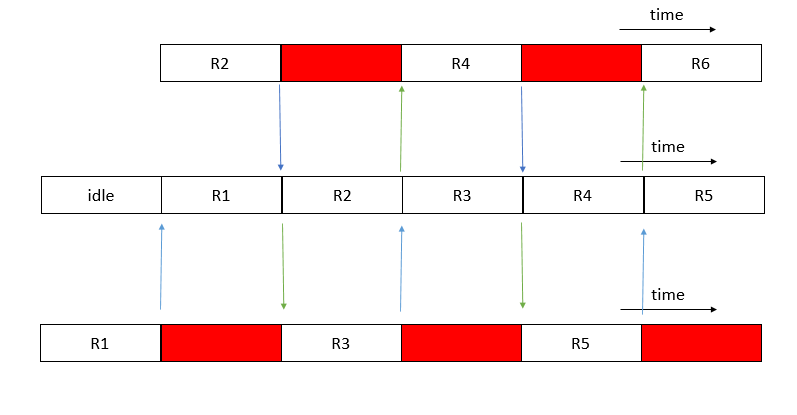
\includegraphics[scale=0.3]{figure/serverview.png}
%	\end{figure}
%\end{frame}



